%% The following is a directive for TeXShop to indicate the main file
%%!TEX root = ../diss.tex

\chapter{Oxygen enhanced MRI}
\label{ch:oemri1}

\section{Preface}

With the exception of Sections~\ref{sec:numComponents},~\ref{sec:correctionfactor}, and \ref{sec:interleave} material presented in this chapter was published in the \textit{Journal of Magnetic Resonance in Medicine}.
Details of co-author contributions appear in the Preface (~\ref{ch:preface}).

% ======================================================================
\section{Introduction}
% ======================================================================

Hypoxia is a well-established component of the tumour microenvironment, arising most often as tumour cell proliferation outpaces the growth of new vasculature.
tumour hypoxia is an indicator of poor prognosis and is responsible for tumour resistance to radiotherapy and some chemotherapies, but is also a potentially useful target for novel anti-cancer drugs~\cite{Wilson:2011jp}.
Assessing tumour hypoxia in the clinical setting is challenging largely due to the invasive nature of biopsy-dependent techniques and the limited capacity and high expense of the more favored, non-invasive PET imaging of hypoxia tracers~\cite{Horsman:2012kw}.
The utility of screening patients for hypoxia was demonstrated retrospectively in trials of the hypoxic cytotoxin tirapazamine, where those patients with greater PET-imaged hypoxia experienced greater benefit ~\cite{Rischin:2006fz}.
However, subsequent trials of drugs targeting hypoxia, including those for evofosfamide that failed to show clinical benefit, have not used hypoxia imaging to stratify patients.
A practical, widely applicable, and non-invasive imaging method is urgently required as a biomarker to monitor tumour hypoxia in many contexts, and is crucial to the development and clinical evaluation of future hypoxia-targeting drugs.

The T$_1$ shortening property of oxygen dissolved in fluid has been known since 1955~\cite{Chiarotti:1955kf} and pioneering work by Young et al. showed that oxygen acts as a paramagnetic contrast agent by demonstrating its ability to reduce T$_1$ upon inhalation~\cite{Young:1981vf}. 
Inhalation of 100\% oxygen has also been shown to elicit strong T$_1$ effects in the kidney\cite{Jones:2002dh}, spleen\cite{Tadamura:1997vc} and the poorly oxygenated retina~\cite{Berkowitz:2001uz}. 
Subsequent oxygen-enhanced MRI (OE-MRI) efforts have included either acquisition of quantitative T$_1$ maps before and after oxygen breathing, or acquiring dynamic T$_1$-weighted (T1W) signal intensity images and calculating $\Delta$T$_1$ during periods of oxygen inhalation.
The subtle but measurable influence of tissue oxygenation on T$_1$ in tumours has been reported by O'Connor~\cite{OConnor:2016ee,OConnor:2009ku,OConnor:2009bp,Little:2018iu}, Mason~\cite{Zhao:2015ez,White:2016fz,Hallac:2014cb}, Gallez~\cite{Jordan:2012do}, and others~\cite{Tadamura:1997vc,McGrath:2008kx,Kershaw:2010ha,Linnik:2013hf}. 
However, due to the changes in T$_1$ that arise as oxygen dissolves in the plasma and interstitial fluid being quite small, T$_1$ maps have poor sensitivity and application of OE-MRI techniques in cancer has yielded mixed success.
OE-MRI continues to suffer from low SNR and it has not found routine clinical use largely because isolating small signal changes due to dissolved O$_2$ is a challenge~\cite{OConnor:2016ee, Zhao:2015ez}.

Typical imaging times for existing OE-MRI methods range from 20-45 minutes often making it impractical for easy inclusion in experimental protocols. 
An MRI technique measuring tumour oxygenation that is sensitive, fast, flexible, repeatable, and non-invasive has the potential to significantly impact the clinical fields of radiation biology and hypoxia drug targeting.
In this study, we present a new dynamic OE-MRI (dOE-MRI) method that allows extraction of very small dynamic signal changes in T$_1$W images by inducing step changes in the inspired oxygen through a repeated, cycling gas challenge.
To isolate the signal component that matches cycling gas, a machine-learning approach called independent component analysis (ICA) is used to analyze MR images as first proposed by McKeown at al~\cite{McKeown:1998wo}.
ICA is a form of blind source separation algorithm that separates the additive signals on the basis of the statistical independence of individual components~\cite{Hyvarinen:2000vk}.
With the application of a cycling oxygen challenge and processing the data using ICA, our dOE-MRI approach represents a significant improvement in the sensitivity and application of MRI for measuring tumour oxygenation, making it more practical for wide application.
% ======================================================================
\section{Methods}
% ======================================================================
\subsection{Mice and tumours}

All animal experimental procedures were carried out in compliance with the guidelines of the Canadian Council for Animal Care and were approved by the institutional Animal Care Committee. 
Female NRG mice were implanted with murine squamous cell carcinoma SCCVII tumours (5 x 10$^5 $cells in 50 $\mu$l serum-free media; cells provided by Dr. J Evans) or with human colorectal carcinoma HCT-116, human ovarian carcinoma SKOV3 or human breast carcinoma BT-474 tumours (each as 10 x 10$^6 $cells in 50 $\mu$l serum-free media; cell lines obtained from the American Type Culture Collection) and were imaged when the largest tumour diameters reached approximately 8-10 mm.
Mice were anesthetized with isoflurane for the duration of imaging sessions until euthanasia, and were positioned supine on the custom surface coil apparatus.
Throughout the imaging session, a small animal monitoring system (SAII Instruments, Stony Brook, NY, USA) was used to monitor respiration rate, varying between 80-100 breaths per minute, and body temperature, maintained at 36.8 $\pm$ 0.5$^\circ$C using a continuous airflow heater.
All animals were injected with 60 mg/kg pimonidazole hydrochloride (HypoxyProbe) 30 min prior to imaging to label hypoxic cells and were euthanized within 15 min of imaging completion.
tumours were embedded and frozen in optimum cutting temperature medium (OCT; Tissue-TEK).

\subsection{Immunohistochemistry, image acquisition and analysis}
Co-planar MRI slices and histological sections were obtained by imaging perpendicular to the longest tumour axis in MRI and serial-step 10 $\mu m$ cryosections were cut at 0.5-mm intervals in the same plane.
Slides were then fixed in acetone-methanol for 10 min and whole sections were immunohistochemically stained~\cite{Kalra:2017is} for CD31 (PECAM; visualized using secondaries labeled with Alexa 647nm) to label blood vessels, and for pimonidazole (HypoxyProbe-1; visualized using secondary labeled with Alexa 546nm) to label hypoxic cells. Sections were then stained using Hoechst 33342 (bisbenzimide) to label all cell nuclei.
Whole-tumour sections were imaged using a robotic fluorescence microscope (Zeiss Axioimager Z1), a cooled, monochrome CCD camera (Retiga 4000R; QImaging), a motorized slide loader and x-y stage (Ludl Electronic Products) and customized ImageJ software~\cite{Collins:2007jr}. 
Adjacent microscope fields of view were tiled such that images of entire tumour cryosections were captured at a resolution of 1.5 $\mu m$/pixel. 
Using anatomical landmarks and accumulated thicknesses of serial-step sections as estimates of distances from the edges of whole tumours, sections were chosen to match the MR slices. 
ImageJ and user-supplied algorithms were used to super impose digital images which were then manually cropped to tumour tissue boundaries with staining artifacts removed. A threshold was applied to images to identify positive pimonidazole staining, and the number of positive pixels was determined as a percentage of the total number of pixels in the tumour image. The histological hypoxic fraction is reported in the highly necrotic HCT-116 tumours as the percentage of pimonidazole+ pixels summed with the percentage of necrotic pixels, as this value should most closely approximate the MR imaging data that does not discriminate between these regions; SCCVII tumours do not have necrosis and so the same value is reported as the percentage of pimonidazole+ pixels.
Overlaid greyscale images were converted to false color for visualization with pimonidazole as green and CD31 as magenta. 

\subsection{MRI Data Acquisition}
All MRI experiments were performed at the UBC MRI Research Centre on a 7T Bruker BioSpec 70/30 scanner at room temperature with a volume transmit coil and custom surface receive coil.
Each imaging session began with pilot axial and coronal T$_2$W scans for tumour localization and slice prescription.
Eight contiguous axial slices (1mm thickness) were acquired with an in-plane field of view of 3.84 cm x 1.92 cm and a matrix size of 128 x 64.
Dynamic oxygen enhanced MRI (dOE-MRI) scans were acquired with a 2D multi-slice FLASH-based sequence with TE/TR = 2.67ms/66.7 ms, $\alpha$ = 40$^\circ$, temporal resolution of 4.3s with 198 repetitions for a total scan time of about 14 minutes.
The spatial resolution and geometry for all scans in the imaging session were matched and an experienced operator outlined the tumour on each slice of the anatomy MR images to construct the region of interest (ROI) for each animal.

\noindent\textbf{Gas challenge during MRI:} tumour-bearing mice began the dOE-MRI gas challenge breathing medical air and were switched between 100\% oxygen and medical air in two-minute intervals.
This paradigm continued for three cycles over a total of fourteen minutes; gases were switched manually and each switch took about five seconds to complete.

\subsection{MRI Data Analysis}
\textbf{dOE-MRI maps:} A suite of in-house software was developed using the python machine learning library scikit-learn~\cite{Pedregosa:2011tv}, specifically \texttt{sklearn.decomposition.FastICA} based on the technique described by Hyvarinen~\cite{Hyvarinen:2000vk}.
The FastICA algorithm is applied to serially acquired T$_1$W images and the output is a paired set of components and weighting factors for each voxel in the dataset.
Extracted independent components are not ordered and while the component selection can be automated, in this study an observer was assigned to select the appropriate component (Figure~\ref{technique}).
The number of independent components for each imaging session was chosen by the operator and ranged from 4-9 to ensure the cyclic behaviour of the T$_1$W signal intensity corresponding to the gas challenge appeared in only one component. 
The dOE-MRI maps were obtained by dividing the ICA weighting-factor maps by the mean signal-intensity maps to obtain a spatial map for the strength of a particular voxel's contribution to the component of interest ($c_4$ in Figure~\ref{technique}).
In these dOE-MRI maps, voxels are coloured to indicate the amount by which a given pixel intensity timecourse is modulated by the oxygen-related component.  
The green-white-purple colour spectrum depicts the degree to which voxels respond to the cycled gas challenge.
Purple indicates O$_2$-positive voxels whose timecourse exhibits a higher and more positive contribution from the corresponding ICA component, representing an increase in T$_1$W signal intensity in response to the supplied 100 \% oxygen, and corresponding to areas with excess dissolved oxygen. 
O$_2$-negative voxels that show a decrease in T$_1$W signal intensity with a negative contribution from the corresponding ICA component under 100 \% oxygen breathing are depicted as green. 
Regions whose T$_1$W signal intensity timecourses responds only weakly or not at all to the gas challenge are shown in white hues.
Fraction of voxels that are negative on dOE-MRI maps were correlated with the histological hypoxic fraction using Pearson's r.

\noindent\textbf{OE-MRI without ICA:} To assess whether or not ICA was necessary to create oxygenation maps, the MR signal intensity data was correlated with two modeled paradigms: 1) a square wave which corresponds to the concentration of delivered oxygen; 2) a synthetic hemodynamic response function (HDRF) created by convolving a square wave with an exponential ($\tau=0.32$ms).
Correlations were calculated voxel by voxel using:

\begin{equation}
r = \frac{\Sigma^n_{i=1} (x_i - \bar{x}) (y_i - \bar{y})}{\sqrt{\Sigma^n_{i=1} (x_i - \bar{x})^2 \Sigma^n_{i=1} (y_i - \bar{y})^2}}
\end{equation}
where $x$ is the model paradigm and $y$ is the T$_1$W signal intensity timecourse.
The resulting correlation maps are estimates of the strength of the input paradigms with the acquired signal intensity.

% ======================================================================
\section{Results}
% ======================================================================

\subsection{ICA isolates small changes in T$_1$W signal intensity}

An example signal intensity vs.\ time curve is shown for a whole slice ROI compared with a single voxel (Figure~\ref{technique}B).
A mean signal intensity increase is seen for both the whole slice and the individual voxel during each of the oxygen periods of the cycle, however the magnitude of $\Delta SI$ for the individual voxel is about 10\% and the noise is of the same order of magnitude.
The slice-averaged timecourse has much less noise compared to the individual voxel, but the size of the effect is also reduced and the contrast to noise is similarly poor.
ICA was then applied to the same dataset and in this example, four independent components were extracted (Figure~\ref{technique}C). 
Each individual independent component is scaled such that its norm is one ($||c_i||=1, \forall i $).
Corrupting influences are often present such as temperature drifts yield slowly increasing or decreasing trends (for e.g., $c_1$), artefacts resulting from slight sub-pixel motion near the edges of the tumour ($c_2$) and breathing artefacts corresponding to short-lived spikes ($c_3$).
Only one extracted component follows the step function of the oxygen challenge and positively identifies an effect of oxygen breathing (c$_4$).
\begin{figure}[htbp]
   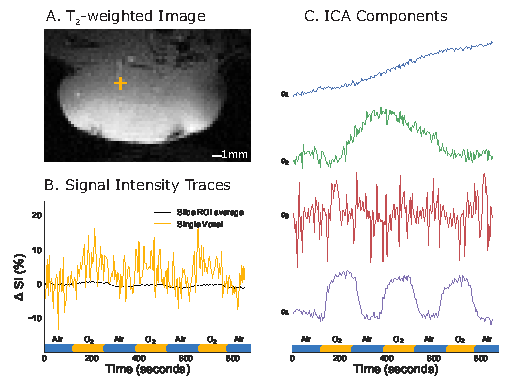
\includegraphics[width=\textwidth]{oemri_thesis1/oemri_thesis1-images/fig1_technique.pdf} % requires the graphicx package
   \caption{(A) T$_2$W MRI of a tumour xenograft at 7T and (B) the corresponding T$_1$W signal-time traces of a single voxel (solid yellow) and whole-tumour slice ROI (dotted black) during gas cycling at two-minute intervals of air (x axis; blue) and O$_2$ (x axis;yellow).
(C) Plot of the four extracted ICA components from the entire tumour ROI, component \textbf{$c_4$} (purple) exhibits the same temporal features as the oxygen cycling time course shown along the bottom. All components are normalized, no vertical scale is shown.}
   \label{technique}
\end{figure}

\subsection{dOE-MRI with ICA does not require assumption of a response function}
To determine whether dOE-MRI maps obtained with a model-free ICA approach (Figure~\ref{fig_correlation}A) are comparable to maps assuming a mathematical model of the response, alternative oxygenation status maps were constructed. 
In Figure~\ref{fig_correlation}B and C, two example mathematical models - a square wave and the estimated hemodynamic response function (HDRF) - are correlated to the voxel-by-voxel raw time signal. 
Regions most correlated with the input paradigm remained purple in both alternative maps generated from modeled response functions.
Particularly when using the HDRF, the alternative oxygenation map showed very similar patterns in the regions demarcated as O$_2$-positive and O$_2$-negative. 
However, the map generated from correlating a square wave led to consistent underestimation of oxygenation relative to the model-free dOE-MRI map.

\begin{figure}[htbp]
   \centering
   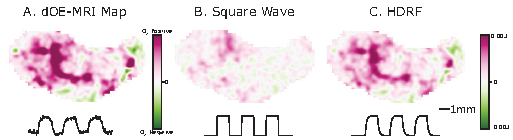
\includegraphics[width=\textwidth]{oemri_thesis1/oemri_thesis1-images/fig3_correlation.pdf} % requires the graphicx package
   \caption{(A) dOE-MRI map of an SCCVII tumour where purple voxels contribute strongly to the extracted component using ICA in the T$_1$W signal timecourses. 
Green voxels in the dOE-MRI map have a strong contribution of the inverse extracted component. Pearson's r-maps are shown correlating the raw time-signal voxel by voxel with a square wave (B), and an exponential convoluted with a square wave called the hemodynamic response function (HDRF) (C).
   \label{fig_correlation}}
\end{figure}

\subsection{Extracting the cycling component via ICA is independent of number of components}
\label{sec:numComponents}
dOE-MRI maps from ICA applied serially after varying the number of components ($m$) from 3 to 12 are shown in Figure~\ref{numComponents}.
The component of the signal that corresponds to the T$_1$W signal intensity increase due to the cycling oxygen is quite prominent and independent of the number of components selected.
Two examples are shown, with a low and high degree of variability measured in the extracted components.
In both cases, the corresponding dOE-MRI maps show the same O$_2$-positive and O$_2$-negative regions.

\begin{figure}[htbp]
   \centering
   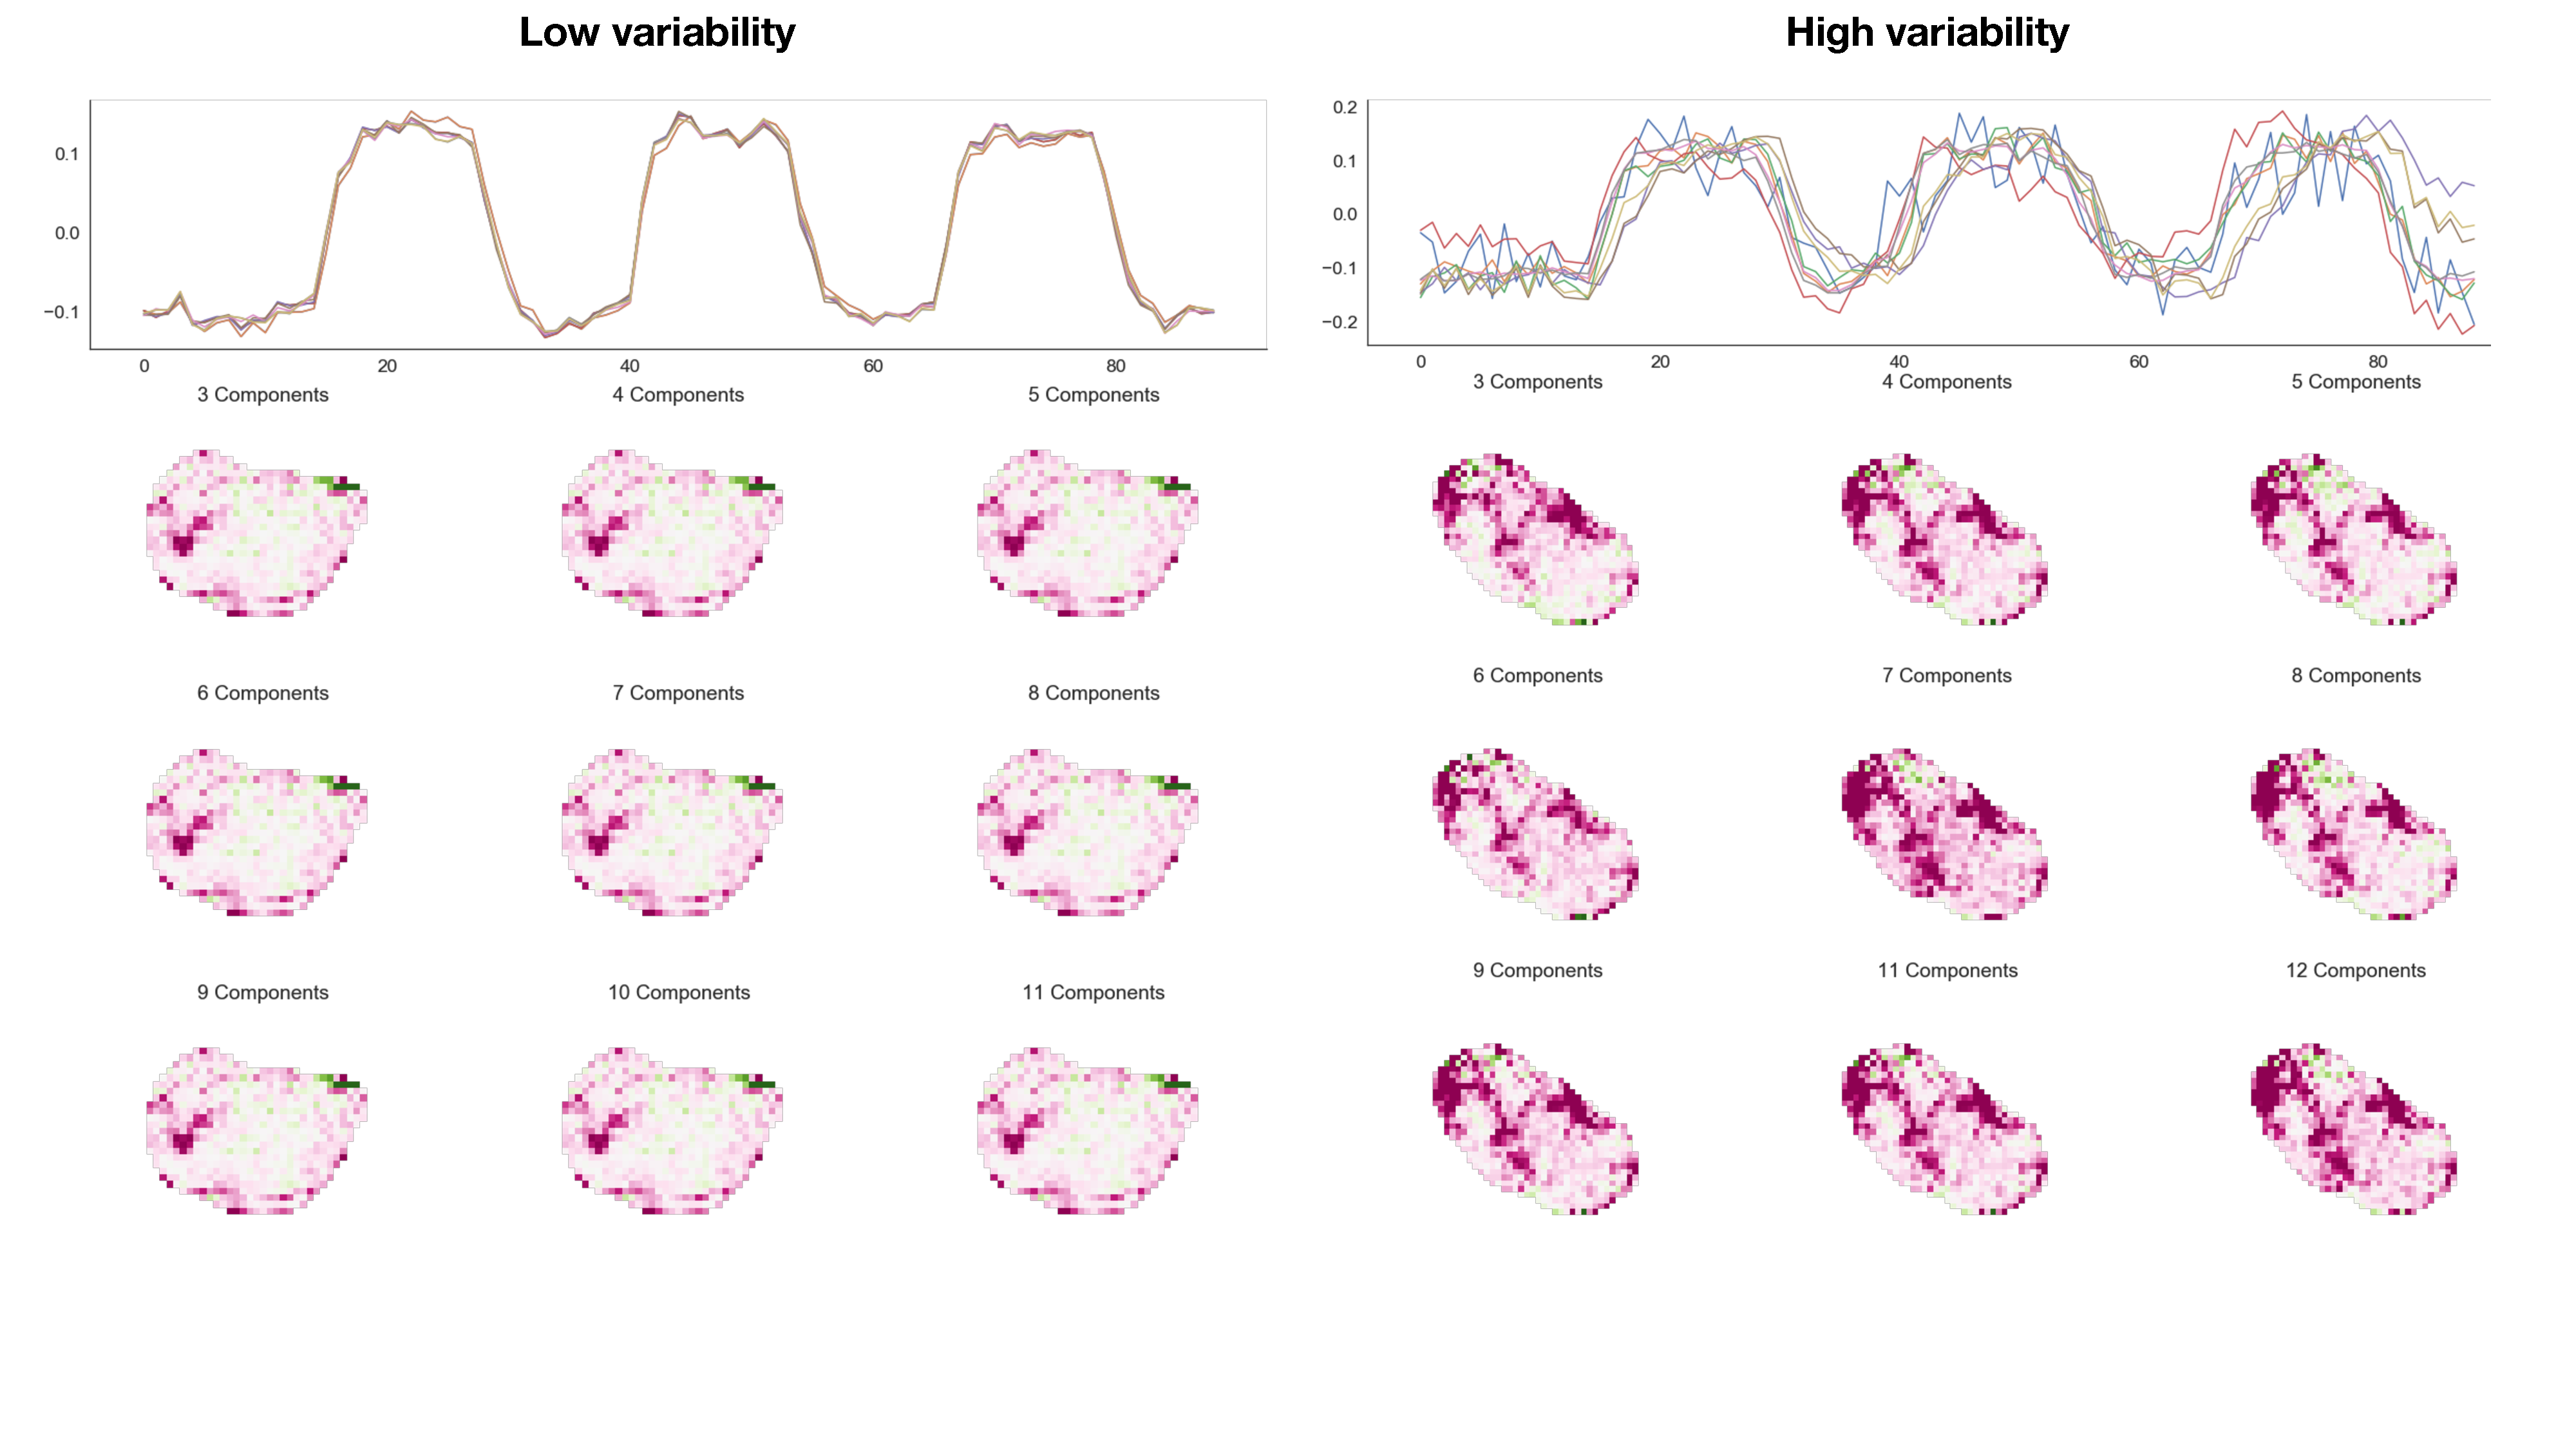
\includegraphics[width=\textwidth]{oemri_thesis1/oemri_thesis1-images/technical_numComponents.pdf} % requires the graphicx package
   \caption{Two animals were chosen to demonstrate the effect of the number of components ($m$) on the dOE-MRI maps. The low variability example shows no discernible difference in the extracted component anywhere from $m=3$ to $m=12$. The high variability example shows shows considerably more noise in the extracted component, but the same overall trend. The corresponding dOE-MRI maps for both the low variability and high variability examples show almost no difference in the oxygenation maps.}
   \label{numComponents}
\end{figure}

\subsection{Variability of response in individual oxygen cycles}

A full dOE-MRI sequence involved three cycles of oxygen but to assess the potential for shortening the sequence we also separately applied ICA to each of the three oxygen cycles independently.
Separate dOE-MRI maps, as well as voxel-wise correlation plots of a representative SCCVII tumour, are shown in Figure~\ref{fig_repeatability} with Pearson's r$_{all-1}$=0.74,r$_{all-2}$=0.86,r$_{all-3}$=0.84.
Pearson's r ranged from 0.79 to 0.87 for a similar analysis in a representative HCT-116 tumour.

The stability of the independent component extraction was assessed by undersampling the full timecourse threefold prior to application of ICA, and a high correlation between the dOE-MRI maps from full and three-fold undersampled timecourses is observed (Figure~\ref{fig_repeatability}E; Pearson's r = 0.84). 

\begin{figure}[htbp]
   \centering
   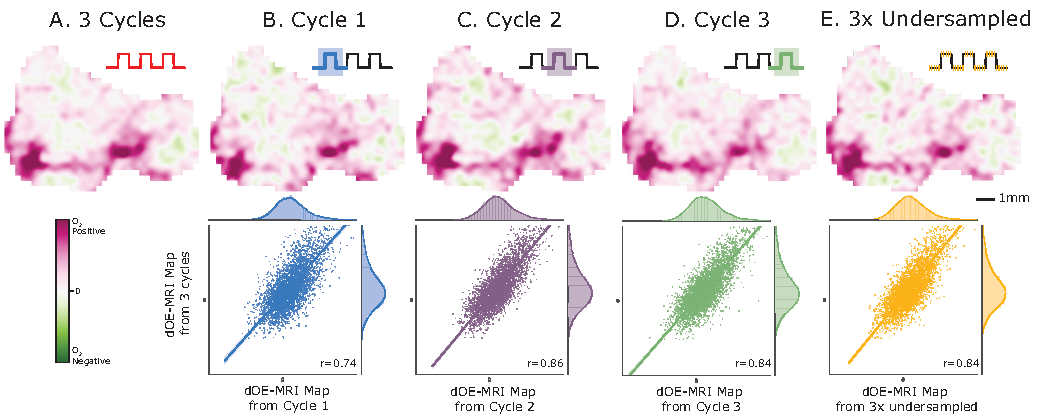
\includegraphics[width=\textwidth]{oemri_thesis1/oemri_thesis1-images/fig4_repeatability.pdf} % requires the graphicx package
   \caption{The dOE-MRI map including the full dataset of all three cycles (A) is compared to each of the three gas cycles separately (B,C,D), and to a map that temporally undersamples by selecting every third datapoint from the full dataset (E).
Voxel-wise plots of each map are correlated to the full dataset and a linear regression with Pearson's r is shown.
   \label{fig_repeatability}}
\end{figure}

\subsection{Comparing oxygen responsiveness with dOE-MRI across experiments}
\label{sec:correctionfactor}
It is possible to compute fractions of positively responding and negatively responding voxels as a surrogate for oxygen responsiveness in tumours with dOE-MRI.
However, this semi-quantitative metric relies on a binary classification of voxels as either O$_2$ positive or O$_2$-negative.
Calculating fractions is sufficient to broadly categorize tumours as oxygenated or not but consequently, rich information about the level of response is lost.
Here we present a new dOE-MRI analysis method that captures the level of response and furthermore, allows direct comparison of data acquired at varying temporal resolutions.

Since each extracted ICA component is scaled such that its norm is one ($||c_i||=1, \forall i $), weighting factor maps are only directly comparable between scans if dOE-MRI images are acquired at the same sampling frequency over the duration of the cycling oxygen (14 minutes).
However, holding the sampling frequency fixed over different experiments is not practical as imaging tumours of different sizes require modification of the field of view and consequently, temporal and spatial resolutions.
A scaling factor (equation~\label{correctionfactor}; derived in the Appendix) must be applied to scale component map values so they can be compared between scans of different temporal resolutions,

\begin{equation}
s = \frac{\sqrt{N_{ref}}}{\sqrt{N}}
\label{correctionfactor}
\end{equation}

A reference sampling frequency should be chosen and in this study, it was chosen to be 0.24s$^{-1}$ (corresponding to N=198 images over the cycling oxygen).

Gas delivered to mice switches between room air and 100\% oxygen in two minute cycles, for a total of 14 minutes.
ICA extracts the tissue response to the delivered oxygen, and four periods of room air interspersed with three periods of oxygen can be modelled mathematically using a general Heaviside function:

\begin{equation}
y(t) =
  \begin{cases}
                                   +b & \text{if $t\geq \frac{3a}{7}$} \\
                                   -b & \text{if $t< \frac{4a}{7}$} \\
  \end{cases},
\end{equation}

For N data points, each $t_i = \frac{ia}{N}$.

The FastICA algorithm places a condition on the norm of the extracted component $y(t)$,

\begin{equation}
\sqrt{\sum_{i=1}^{N} \Bigl|y(t_i)\Bigr|^2} %\coloneqq 1.
\end{equation}

Simplifying the expression above for our $y(t)$, we have:
\begin{align}
1 = \sqrt{b^2 \sum_{i=1}^{N} 1^2} \nonumber \\
b = N^{-\frac{1}{2}}
\end{align}

With this, we can compute the scaling factor directly using b$_{ref}$ =198 repetitions as the reference:

\begin{align}
s = \frac{b_{N}}{b_{ref}} \nonumber \\
s = \frac{\sqrt{198}}{\sqrt{N}} 
\end{align}

This scaling factor was applied to all dOE-MRI maps used in this study to retain information about the level of response to the supplied oxygen across scans with different sampling frequencies.

%\begin{figure}[htbp]
%   \centering
%   \includegraphics[width=0.6\textwidth]{oemri2/oemri2-images/schematic.png} % requires the graphicx package
%   \caption{example caption}
%   \label{dOEMRImaps}
%\end{figure}

%======================================================================
\section{Discussion}
% ======================================================================

Here we present an improved method for OE-MRI that employs two synergistic techniques to achieve higher speed and greater sensitivity.
First, a repeated gas challenge is used to probe tissue response by introducing an independent signal modulation unrelated to nuisance contributions such as temperature drifts and motion.
A repeating gas challenge improves the detection sensitivity of small amplitude signal changes that are typical of oxygen-enhanced MRI.
Second, a repeating signal modulation enables further improved sensitivity through the use of ICA, a signal processing technique to isolate source signals - T$_1$W changes due solely to the cycling oxygen - without knowledge of the tissue response (Figure~\ref{technique}).
While it is possible to generate correlation maps of the oxygen cycling paradigm with T$_1$W signal changes that appear very similar to dOE-MRI maps, an \emph{a-priori} assumption of a response function is required for this approach (Figure~\ref{fig_correlation}).
Furthermore, presupposing a particular oxygen response function biases the identification of responding O$_2$-positive voxels (Figure~\ref{fig_correlation}) underscoring the need for a model-free approach to extracting the oxygen-responding component.

The improved sensitivity of our technique results in broader applicability of dOE-MRI, as we found that an oxygen-enhancing component was extracted successfully in all imaged animals across a range of tumour models and environments (Figure~\ref{versatile}).
The unambiguous match of the identified component with the periods of the gas cycles increases the confidence that the small T$_1$W signal changes result from increased oxygen dissolved in the plasma and interstitial tissue fluids.
Maps from other extracted components (Appendix Figure~\ref{Sfig_components}) exhibit spatial patterns that could provide clues to the signal sources but associating meaning to them is challenging and would require additional data.
For example, even moderate shifts in temperature could drive a measurable change in T$_1$W signal during the timecourse, and a physiological monitoring system that is time-synced to the MR acquisition could illuminate this confounding variable. 
Nevertheless, we have established reliability of the technique by comparing maps from each cycle of the gas challenge to the map incorporating data from all three oxygen-cycles and have found no significant differences.
In fact, the strong correlations between dOE-MRI maps from each of the individual cycles of the gas challenge (Figure~\ref{fig_repeatability}) show that it is feasible to assess tissue oxygenation within 6 minutes.
Performing this analysis again with three-fold temporally under-sampled data suggests that there is sufficient SNR to successfully extract the oxygen responsive component (Figure~\ref{fig_repeatability}) with even a subset of the data.\todo{link this back to the new figure showing you can go up to 6}

dOE-MRI offers a versatile technique where the duration of the cycles and gas challenge, temporal resolution and desired signal-to-noise can be modified based on the imaging objectives, which could include investigating intermittent perfusion or intervention-mediated changes in the tumour microenvironment. 
Of note, supplying excess oxygen to hypoxic tumour cells over time has the potential for increasing the baseline oxygen concentration, effectively reducing the hypoxic fraction and altering the tumour microenvironment~\cite{Linnik:2013hf}.
This would result in voxels becoming more oxygen responsive over progressive oxygen cycles and would depend on the tumour characteristics as well as the duration of the oxygen challenge.
This was not observed on the time scales in our study when using ICA to extract changes in T$_1$W signal intensity just due to the gas challenge. 
Should it arise in other contexts it could possibly be mitigated by extending the air-breathing part of the cycle, or by extracting that as a separate component using ICA.
The potential for creating a hyperoxia steady state by modulating oxygen duration is discussed further by Losert et al ~\cite{Losert:2002gt}.

Depending on the application of dOE-MRI, quantitative O$_2$-positive and O$_2$-negative fractions can be obtained from dOE-MRI maps as shown in this study, by deploying group ICA techniques~\cite{Calhoun:2009jr}, or setting significance thresholds using a t-test~\cite{Greicius:2004ck} and computing z-scores~\cite{McKeown:1998wd}.
To help understand the oxygen dynamics in tumours, including the effect of hemoglobin with T$_2^*$ mapping, fitting exponential recovery and decay curves to the extracted oxygen response curves may provide additional insights as originally proposed by Losert et al. in the brain~\cite{Losert:2002gt}.
In a promising study, White et al. has shown that OE-MRI may be very relevant in developing prognostic factors to predict tumour response to hypofractionation by stratifying tumours that may benefit from oxygen breathing during irradiation~\cite{White:2016fz}.
Featherstone et al. have recently explored pre-clinical datasets using feature-extraction and clustering analysis and this may prove fruitful in understanding the behavior of subregions within a tumour microenvironment~\cite{Featherstone:2018cn}.
Future work to evaluate the utility of dOE-MRI will ultimately depend on its context-dependent validation as a relevant measure of tumour hypoxia to dynamically characterize the clinically relevant oxygen status of tumours, relating this information to treatment sensitivities and outcomes.

% ======================================================================
\section{Conclusions}
% ======================================================================
In this study we extend existing oxygen-enhanced MRI techniques by adding a cycling element to the respiratory challenge and using a blind-source separation signal processing technique (ICA) to extract the oxygen responsive component and responding voxels.
This dOE-MRI method presents significant improvements to the sensitivity and applicability of OE-MRI where small changes in T$_1$W signal intensity arising from cycling respiratory challenges can be separated robustly. Traditional quantitative T$_1$ mapping techniques have longer imaging times and are impractical for OE-MRI due to SNR and time constraints.
dOE-MRI with ICA is clinically translatable as the sequence acquisition is relatively short and most centers already have access to dynamic T$_1$W MRI acquisitions that many patients already routinely receive. 
Therefore dOE-MRI is an exciting, non-invasive and widely available technique for assessing tumour oxygenation that could provide a crucial tool in the field of radiation oncology and in the development of treatments targeting the tumour microenvironment.

% ======================================================================
\section{Acknowledgments}
% ======================================================================

Dr. Martin McKeown provided assistance in understanding the utility of ICA in the given context. Dr. Alastair Kyle undertook foundational work by designing and building the microscope and histology acquisition system. 

\section{Appendix}

\subsection{Other independent components extracted}

Figure~\ref{Sfig_components} shows the extracted independent components and their corresponding weighting factor maps for an application of ICA on a OE-MRI scan.
Extracted components typically have a mix of high and low frequency responses and may include temperature drifts, breathing artefacts and other motion. 
Additional physiological monitoring data is needed for a more thorough analysis of the other independent components and whether they can aid our understanding of the mechanism of action.

\begin{figure}[htbp]
   \centering
   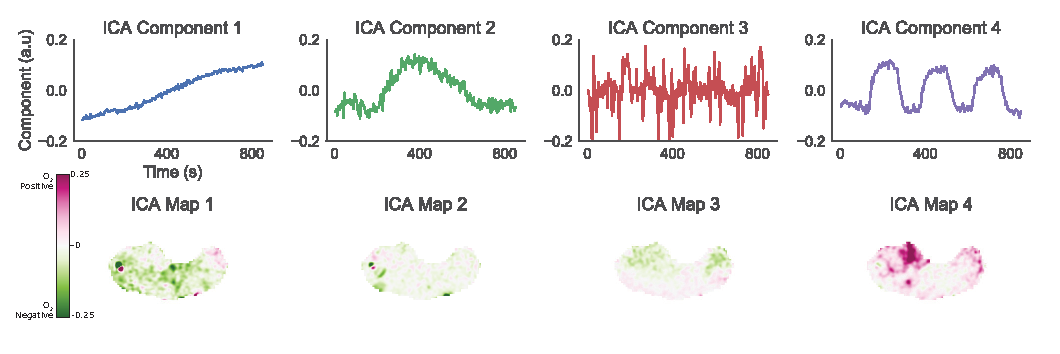
\includegraphics[width=0.9\textwidth]{oemri_thesis1/oemri_thesis1-images/fig_components.pdf} % requires the graphicx package
   \caption{Plots of the four components extracted from ICA are shown (($||c_i||=1, \forall i $) along with the corresponding  weighting factor maps (normalized to mean voxel wise mean signal intensity). Note that c$_4$ is clearly the component of interest here as the cycling pattern is not present in any other component. We speculate that c$_1$ corresponds to a temperature drift over the course of the scan and c$_3$ is likely related to a breathing motion artefact. Component 2 is a relatively weak spurious signal fairly low in magnitude with no obvious spatial or temporal pattern. Further investigation is required to explore the underlying physiological response (if any) of the other components.
   \label{Sfig_components}}
\end{figure}

\subsection{Subsampling - can interleave with T2*}
\label{sec:interleave}
Another example showing the dOE-MRI maps extracted using ICA using a subset of the same source data.
This example more clearly highlights the low variation 


Mauris ultrices, nibh in rutrum eleifend, nisl sapien suscipit ipsum, finibus imperdiet metus tellus in nunc. Fusce eget tellus tincidunt lectus convallis elementum quis sed ante. Nullam nisl tellus, gravida nec arcu nec, bibendum finibus ipsum. Proin eu turpis quam. Sed faucibus, urna id consequat placerat, enim ligula porttitor velit, id congue eros elit a eros. Sed pharetra nunc rutrum massa auctor iaculis. Interdum et malesuada fames ac ante ipsum primis in faucibus. Nunc quis sapien lacus. Morbi suscipit sed ante id.

\begin{figure}[htbp]
   \centering
   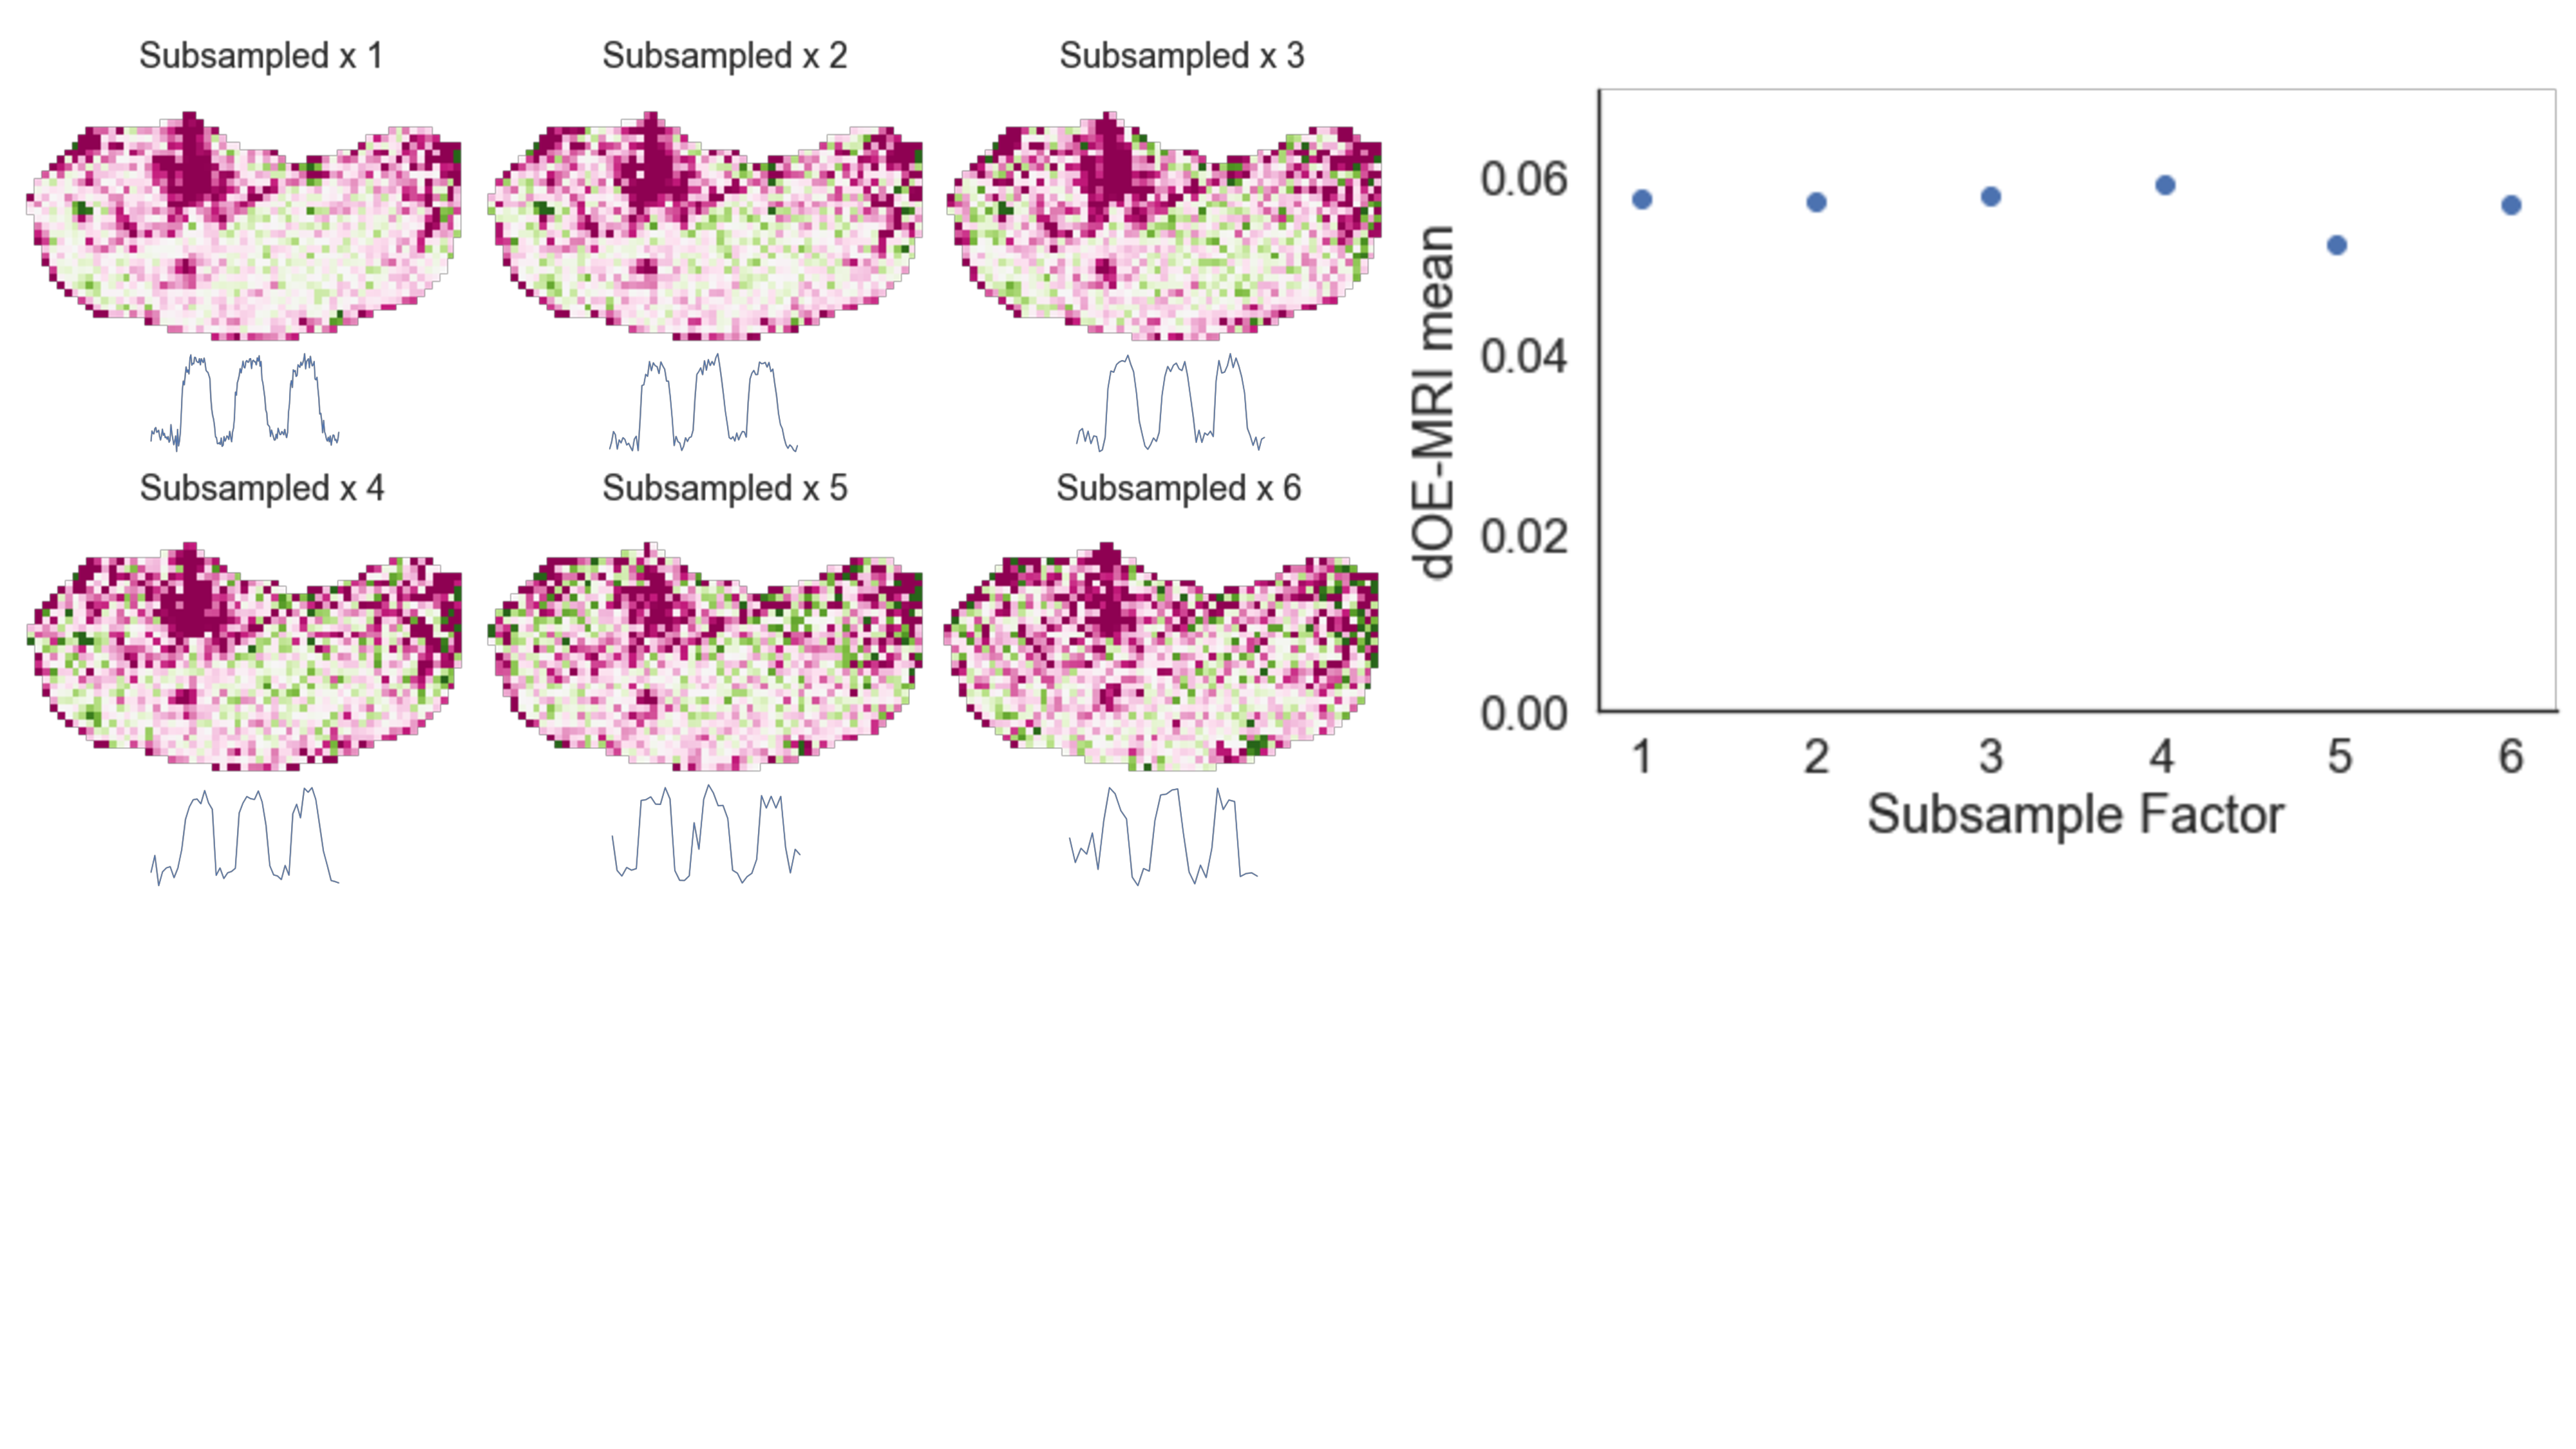
\includegraphics[width=\textwidth]{oemri_thesis1/oemri_thesis1-images/technical_subsample.pdf} % requires the graphicx package
   \caption{dOE-MRI maps and associated component traces of differently sampled data. To achieve different levels of subsampling, the raw data was spliced and then ICA was applied. The oxygenation maps look very similar between different subsample factors. Temporal resolution and number of points were 4.3 s and 200 points (subsample 1), 8.5 s and 100 points (subsample 2), 12.8s and 67 points (subsample 3), 17.1s and 50 points (subsample 4), 21.3s and 40 points (subsample 5), and 25.12s and 34 points (subsample 6).}
   \label{subSample}
\end{figure}

\endinput
